\documentclass{article}

%IDIOMA
\usepackage[spanish]{babel}
\usepackage[latin1]{inputenc}  % Ambos para solucin de asuntos de idioma
\usepackage[T1]{fontenc}

%MATH
\usepackage{amsmath,amssymb,mathrsfs,mathptmx}  % Matemticas varias
\usepackage{hyperref} % Para escribir URLs
\usepackage{verbatim}

%IMAGES
\usepackage{graphicx}
\usepackage{epstopdf}
\usepackage{float}
\usepackage{subfigure}
\usepackage{wrapfig}
\usepackage[usenames,dvipsnames]{color}
\graphicspath{{./figure/}}
\DeclareGraphicsExtensions{.png,.jpg,.pdf,.mps,.gif,.bmp, .eps}
\usepackage{caption}

%VARIOS
\usepackage{multirow}
\usepackage{multicol}
\usepackage{tabulary}
\usepackage[table]{xcolor}
\usepackage{color}
\usepackage{listings}

\usepackage{tikz}


\begin{document}

\title{\Huge HPPS \\ \huge Informe 3 - Ejercicios de grafos}

\author{ Juan Braun}
\maketitle

%\include{intro}
\section*{Introducci�n}
% v5.0: corregida por el tribunal.


El objetivo de este informe es comentar los resultados obtenidos para los ejercicios propuestos. 

\section{Ejercicio 1}
El objetivo de este ejercicio fue hacer un programa para calcular el histograma de grados de todos los v�rtices para un grafo cualquiera de orden \textit{N}.

La entrada al programa es un archivo con la matriz de adyacencia. Para generar este archivo se creo un ejecutable que genera matrices de adyacencia de forma aleatoria. El c�digo fuente para este ejecutable esta en el archivo \verb|adjMat.c|.

Los argumentos a ingresar son el orden del grafo, una bandera para hacer que la matriz de adyacencia sea sim�trica y el nombre del archivo en el que se va a guardar la salida. A continuaci�n se muestra una llamada al ejecutable. 
\begin{verbatim}
./adjMat 4 1 mat
\end{verbatim}

A continuaci�n se muestra la salida de la funci�n que calcula los grados y el histograma.

\begin{verbatim}
size= 4
0 1 1 1 
1 0 0 0 
1 0 0 0 
1 0 0 0 
GRADO
3 1 1 1 
HISTOGRAMA
0 3 0 1 
\end{verbatim}

\section{Ejercicio 2}

El objetivo de este ejercicio fue implementar el algoritmo de b�squeda en profundidad (\textit{DFS}), en sus dos variantes, la version recursiva y la version iterativa. 

Se utilizaron diferentes arboles para probar ambas versiones.

\begin{figure}[h!]
  \centering
    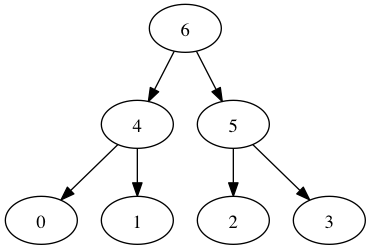
\includegraphics[width=0.3\textwidth]{t1}
    \caption{�rbol de prueba 1(A1)}
\end{figure}

\begin{figure}[h!]
  \centering
    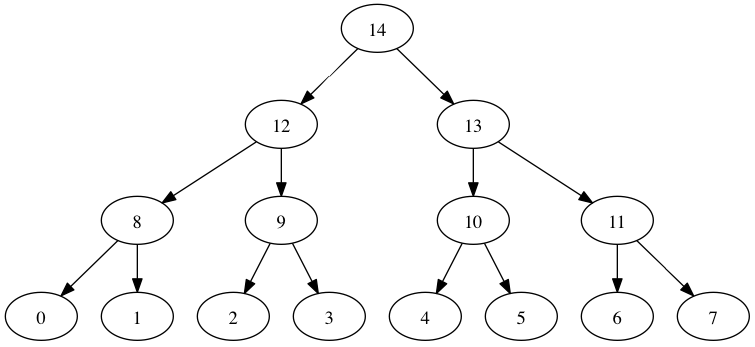
\includegraphics[width=0.5\textwidth]{t2}
    \caption{�rbol de prueba 2(A2)}
\end{figure}

\begin{figure}[h!] 
 \centering
    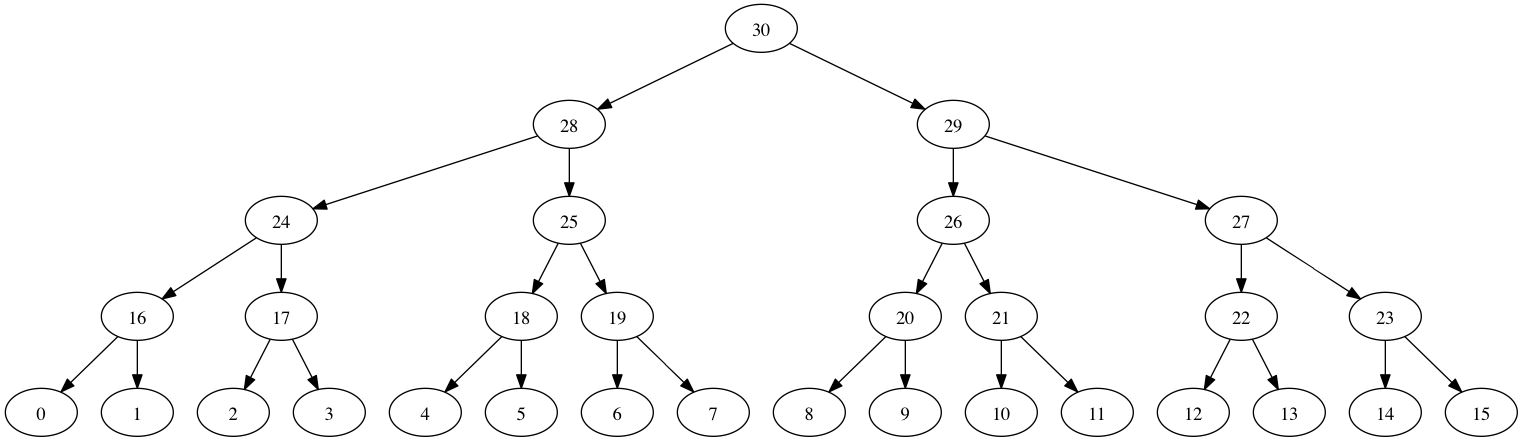
\includegraphics[width=1\textwidth]{t3}
    \caption{�rbol de prueba 3(A3)}
\end{figure}

\begin{table}[h!]
\centering
\begin{tabular}{| l | c | c |}
\hline
 & \verb|dfs_rec| & \verb|dfs_it|\\[0.5ex]
\hline
A1 & 168 & 437\\ \hline
A2 & 376 & 893\\ \hline
A3 & 792 & 1805\\ \hline

\end{tabular}
\caption{Ciclos para versi�n recursiva e iterativa}
\label{table:Ciclos}
\end{table}

Como se puede ver en el Cuadro \ref{table:Ciclos} la versi�n recursiva del algoritmo necesita menos ciclos para realizar la b�squeda. Ademas se verifica que el algoritmo es de orden \textit{O(|E|)} ya que para los diferentes arboles los ciclos crecen linealmente. 

Para entender mejor porque una versi�n requiere menos ciclos que la otra se muestra es pseudo-c�digo de ambas.

\begin{verbatim}
dfs_rec(A,n)

if (n no tiene hijos)
  estoy en el fondo->proceso n
else
  n = primer hijo de n
    dfs_rec(A,n)
    while (n tiene hermanos)
      n = hermano de n
      dfs_rec(A,n)
    end while
    proceso n
end if

end
		
	
\end{verbatim}
\begin{verbatim}
dfs_it(A,n)
 
creo stack Abiertos
creo stack Cerrados
pongo nodo n en stack Abiertos
while(Abiertos no este vacio)
  saco nodo n de Abiertos 
  pongo nodo n en Cerrados
  if (n tiene hijos) 	
    n =primer hijo de n
    pongo a n en Abiertos 
    while(n tiene hermanos)
      n = hermano de n 
      pongo a n en Abiertos
    end while
  end if
end while
 
proceso los nodos en el orden que aparecen en Cerrados		
 
end
\end{verbatim}

Lo primero que se nota a simple vista es el tama\~no de ambos pseudo-c�digos. Si bien la versi�n iterativa es la mas intuitiva, la implementaci�n de esta es mas compleja. Ademas hay que crear stacks para almacenar los nodos que se vistan, por lo que se requiere reservar memoria. Finalmente se procesan los nodos una vez terminada la b�squeda, ya que el stack que se utiliza para guardar los nodos es un stack LIFO.  

En la versi�n recursiva se procesan los nodos a medida que se va recorriendo el arbol. Ademas no se necesita crear ning�n stack para almacenar nodos visitados. 

La diferencia entre la cantidad de ciclos de reloj se debe a la cantidad de movimientos de memoria que se realizan en la versi�n iterativa.  

Cuando se realiza procesamiento sobre los nodos, el desempe\~no de ambas versiones deja de ser tan diferente. En el caso de las pruebas realizadas, se tomo como procesamiento del nodo la acci�n de imprimir el nombre del nodo en pantalla.
Para este caso se puede ver en el Cuadro \ref{table:CiclosPorc} que los ciclos son similares para ambas versiones. 
\begin{table}[h!]
\centering
\begin{tabular}{| l | c | c |}
\hline
 & \verb|dfs_rec| & \verb|dfs_it|\\[0.5ex]
\hline
A1 & 5767 & 6108\\ \hline
A2 & 12601 & 13266\\ \hline
A3 & 26545 & 27858\\ \hline

\end{tabular}
\caption{Ciclos para versi�n recursiva e iterativa con procesamiento}
\label{table:CiclosPorc}
\end{table}

De todas formas se concluye que la versi�n recursiva del algoritmo de b�squeda en profundidad es la m�s eficiente y la m�s elegante.



\end{document}


